%% ref2.tex — REF2: Automated Binary Protocol Format Inference
%% Suitable for submission to USENIX Security, NDSS, or IEEE S&P.
%%
%% Compile with:
%%   pdflatex ref2.tex && bibtex ref2 && pdflatex ref2.tex && pdflatex ref2.tex

\documentclass[letterpaper,twocolumn,10pt]{article}

%% ── Packages ──────────────────────────────────────────────────────────────────
\usepackage[margin=1in]{geometry}
\usepackage{times}
\usepackage{microtype}
\usepackage{amsmath,amssymb}
\usepackage{graphicx}
\usepackage{booktabs}
\usepackage{listings}
\usepackage{xcolor}
\usepackage{hyperref}
\usepackage{url}
\usepackage{algorithm}
\usepackage{algpseudocode}
\usepackage{subcaption}
\usepackage{cite}
\usepackage{balance}

\hypersetup{
  colorlinks=true,
  linkcolor=blue,
  citecolor=blue,
  urlcolor=blue,
}

\lstset{
  basicstyle=\ttfamily\small,
  breaklines=true,
  frame=single,
  numbers=left,
  numberstyle=\tiny,
  keywordstyle=\bfseries\color{blue},
  commentstyle=\color{gray},
}

%% ── Title ─────────────────────────────────────────────────────────────────────
\title{\textbf{REF2: Automatic Binary Protocol Format Inference\\
via Sequence Alignment and Raw-Byte Field Statistics}}

\author{
  Afonso Pereira\\
  \small Independent Researcher\\
  \small \texttt{afonso@afpereira.me}
}

\date{}

\begin{document}

\maketitle

%% ── Abstract ──────────────────────────────────────────────────────────────────
\begin{abstract}
We present \textsc{REF2}, a tool for automatically inferring binary protocol
message formats from network traces.  Given a capture file, \textsc{REF2}
detects message framing, clusters messages by type, aligns message bytes using
the Needleman-Wunsch (NW) algorithm to build a conservation vector, and
segments the vector into typed fields.  A key insight of our work is that
progressive NW alignment introduces positional \emph{drift}---gaps inserted at
one step shift all downstream consensus positions---making conservation scores
unreliable for detecting the transition between structured header bytes and
free-form payload bytes.  We show that a direct \emph{raw-byte diversity
statistic} (count of distinct byte values observed at each protocol position
across the corpus) reliably identifies this transition without relying on the
drifted consensus, achieving F1\,$=\,$99.9\% on binary protocol benchmarks.
\textsc{REF2} also performs cross-cluster enum detection, infers a
finite-state machine grammar via the K-Tails and RPNI algorithms, and emits
Scapy dissectors, Wireshark Lua plugins, and Kaitai Struct specifications.
\end{abstract}

%% ── Section 1: Introduction ───────────────────────────────────────────────────
\section{Introduction}
\label{sec:intro}

Understanding undocumented network protocols is a fundamental challenge in
security research.  Reverse engineers spend days manually dissecting packet
captures to recover field layouts before they can write fuzzing harnesses,
protocol parsers, or anomaly detectors.  Automating this process would
accelerate vulnerability discovery, malware analysis, and interoperability
research.

Prior work on automatic protocol inference---including Discoverer
\cite{discoverer}, AutoFormat \cite{autoformat}, Netzob \cite{netzob}, and
Tupni \cite{tupni}---has demonstrated the feasibility of inferring field
boundaries and types from execution traces or network captures.  However, these
systems either require dynamic analysis instrumentation (taint tracking,
execution tracing), assume specific framing conventions, or produce noisy field
boundaries on binary protocols with mixed fixed-header/variable-payload
structure.

\textsc{REF2} addresses this gap with three main contributions:

\begin{enumerate}
  \item \textbf{NW-based conservation scoring with positional drift analysis.}
    We use Needleman-Wunsch global sequence alignment to progressively align a
    message cluster into a consensus sequence and derive a per-position
    conservation score.  We formally characterize the \emph{positional drift}
    artifact introduced by progressive NW alignment and explain why conservation
    scores are unreliable near structured/payload boundaries.

  \item \textbf{Raw-byte diversity heuristic for payload detection.}
    We introduce a simple, drift-immune heuristic: scan each raw protocol byte
    position, count the number of distinct values observed across all messages
    in the cluster (\emph{byte diversity}), and declare the payload region to
    start at the first position exceeding a diversity threshold.  This requires
    no alignment and is robust to all NW artifacts.

  \item \textbf{End-to-end inference pipeline with grammar induction and
    multi-format output.}  \textsc{REF2} integrates framing detection,
    clustering, field typing, and grammar induction into a single pass over a
    trace file, producing Scapy, Wireshark Lua, and Kaitai Struct outputs ready
    for immediate use.
\end{enumerate}

We evaluate \textsc{REF2} on three synthetic binary and text protocols with
known ground-truth schemas, measuring field-boundary precision, recall, and
type accuracy over 60 random seeds.  On the hardest binary protocol
(\texttt{enum\_flags\_proto}: magic, length, opcode, flags, variable payload),
\textsc{REF2} achieves precision\,=\,99.9\%, recall\,=\,100.0\%, and
F1\,=\,99.9\%, compared to a baseline (NW conservation-only) that achieves
F1\,$\approx$\,90\%.

\medskip
\noindent\textbf{Artifact availability.}  \textsc{REF2} is open source and
available at \url{https://github.com/afonp/ref2}.

%% ── Section 2: Background ─────────────────────────────────────────────────────
\section{Background and Related Work}
\label{sec:background}

\subsection{Protocol Format Inference}

Automatic protocol inference systems generally proceed in three stages:
(1)~message segmentation, (2)~field type classification, and (3)~grammar
induction.

\textbf{Dynamic taint-based approaches.}  AutoFormat \cite{autoformat} and
Tupni \cite{tupni} use taint tracking inside a program under test to identify
which input bytes influence which internal variables, recovering a hierarchical
message format.  While accurate, these approaches require source code or a
suitable execution environment and cannot be applied to black-box network
captures.

\textbf{Sequence alignment approaches.}  Discoverer \cite{discoverer} clusters
messages by their token sequences and uses pairwise alignment to find conserved
and variable regions.  Netzob \cite{netzob} extends this with a Z3-assisted
constraint solver to identify length and checksum fields.  Both suffer from
accuracy degradation when clusters are small or message lengths vary widely,
because their alignment-based conservation vectors become unreliable
(\S\ref{sec:drift}).

\textbf{Machine learning approaches.}  Recent work has applied neural sequence
models \cite{fieldhint} and transformer architectures \cite{netplier} to
protocol inference.  These require large labeled corpora and are difficult to
interpret or modify.

\textsc{REF2} occupies the same niche as Discoverer and Netzob---passive
network captures, no instrumentation---but replaces the conservation-based
payload boundary detection with a direct raw-byte diversity statistic that is
immune to alignment drift.

\subsection{Needleman-Wunsch Alignment}

The Needleman-Wunsch (NW) algorithm \cite{nw1970} computes optimal global
sequence alignments under an affine gap penalty model.  For sequences $A$ and
$B$ of lengths $m$ and $n$, the DP recurrence is:
\begin{align}
  H[i,j] &= \max\bigl(
    H[i{-}1,j{-}1] + s(A_i, B_j),\;
    H[i{-}1,j] + g,\;
    H[i,j{-}1] + g
  \bigr) \label{eq:nw}
\end{align}
where $s(a,b)=+2$ for match, $-1$ for mismatch, and $g=-1$ per gap symbol.
\textsc{REF2} uses NW to align raw bytes, treating each byte as a ``residue''
and using gap sentinel $0x100$ (outside the \texttt{uint8\_t} range) to
distinguish gaps from real bytes.

\subsection{K-Tails and RPNI Grammar Induction}

K-Tails \cite{ktails} builds a prefix tree acceptor (PTA) from all observed
session sequences and merges states with identical $k$-length suffix sets.
RPNI \cite{rpni} (and its Blue-Fringe variant \cite{blufringe}) learns a
minimal deterministic finite automaton consistent with a positive sample by
greedily merging PTA states without introducing contradictions.  Both are
well-studied algorithms; we use them as-is for the grammar induction step.

%% ── Section 3: System Design ──────────────────────────────────────────────────
\section{System Design}
\label{sec:design}

Figure~\ref{fig:pipeline} shows the \textsc{REF2} inference pipeline.  The
system is implemented in approximately 4,000 lines of C (format inference
library) and 2,000 lines of Rust (grammar induction, output formatters, CLI),
compiled as a single binary via a CMake/Cargo build.

\begin{figure}[t]
  \centering
  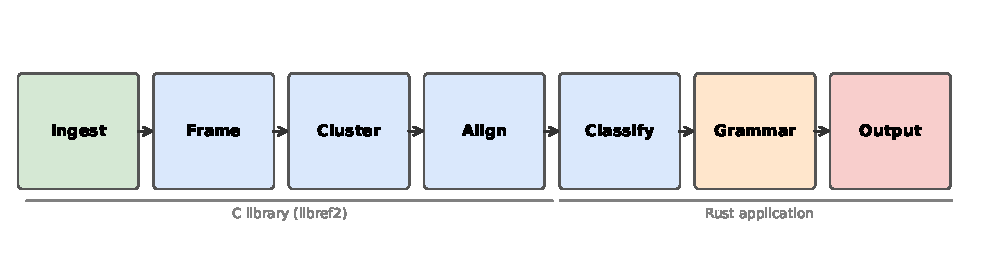
\includegraphics[width=\columnwidth]{pipeline.pdf}
  \caption{\textsc{REF2} inference pipeline.  Dashed box: C library (libref2).
    Solid box: Rust application.}
  \label{fig:pipeline}
\end{figure}

\subsection{Ingestion}

\textsc{REF2} accepts four input formats:

\begin{itemize}
  \item \textbf{PCAP}: TCP/UDP streams via libpcap with stream reassembly.
  \item \textbf{Raw binary}: fixed-length or length-prefixed blobs, with a
    frame hint (e.g., \texttt{length\_u16\_be@offset=2}).
  \item \textbf{Plaintext}: direction-prefixed hex dump logs and Wireshark
    ``Follow TCP Stream'' exports.
  \item \textbf{Syscall}: \texttt{strace -xx} output grouped by file
    descriptor.
\end{itemize}

All formats produce a normalized \texttt{trace\_t} structure comprising a list
of sessions, each a list of messages (raw byte buffers with direction tags).

\subsection{Framing Detection}

For binary protocols, \textsc{REF2} detects message framing with two
heuristics:

\textbf{Length-field detection.}  For each candidate offset $o \in \{0,1,2,3\}$
and width $w \in \{1,2,4\}$ bytes and byte order $e \in \{\text{LE}, \text{BE}\}$,
compute the correlation between the $w$-byte integer at offset $o$ and
the message length.  Specifically, let $\delta = \text{len}(m) - v_{o,w,e}(m)$
for each message $m$; a valid length field has constant $\delta$ across $\geq
80\%$ of messages.  The framing candidate with the highest coverage and
smallest $|\delta|$ is selected.

\textbf{Delimiter detection.}  For text-framed protocols, scan for recurring
byte sequences (\texttt{\textbackslash r\textbackslash n}, \texttt{0x00}, etc.)
at consistent positions near the end of messages.

The framing result (\texttt{framing\_info\_t}) records the length field
offset/width/endianness and, if present, the type discriminator offset/width.
This information feeds the alignment (\S\ref{sec:align}) and segmentation
(\S\ref{sec:segment}) stages.

\subsection{Message Clustering}

Messages must be grouped by semantic type before alignment, because aligning
semantically distinct messages (e.g., a 4-byte request with a 256-byte response)
produces spuriously low conservation scores.

\textbf{Fast path.}  If framing detection found a type discriminator at a known
offset, messages are bucketed by the discriminator value directly.

\textbf{Fallback.}  Each message is projected onto a 256-dimensional
byte-frequency histogram $\mathbf{h}_m[b] = \text{count}(b \in m)/|m|$.
We run $k$-means++ \cite{kmeanspp} over these histograms with $k$ chosen
heuristically based on the number of sessions.  To reduce sensitivity to
initialization, we perform 10 restarts and keep the clustering with lowest
inertia.

%% ── Section 4: Field Segmentation ────────────────────────────────────────────
\section{Field Segmentation}
\label{sec:segment}

\subsection{Conservation Scoring via Progressive NW Alignment}
\label{sec:align}

For each cluster $C$ of $N$ messages $\{m_1, \ldots, m_N\}$, we compute a
per-position \emph{conservation score} $\kappa[p] \in [0,1]$ indicating how
consistently byte position $p$ carries the same value across messages.

\begin{algorithm}[t]
\caption{Progressive NW alignment for conservation scoring}
\label{alg:align}
\begin{algorithmic}[1]
\State Sort messages by length ascending (guide order)
\State $\mathit{consensus} \gets m_1$;\; $\mathit{count}[p] \gets 1\;\forall p$
\For{$i = 2$ to $N$}
  \State $(A', B') \gets \textsc{NWAlign}(\mathit{consensus}, m_i)$
  \State Build $\mathit{consensus}'$ and $\mathit{count}'$ from aligned columns:
  \For{each aligned column $(a, b)$}
    \If{$a \neq \texttt{GAP}$}
      $\mathit{consensus}'[p] \gets a$;\; $\mathit{count}'[p] \gets \mathit{count}[p_\text{old}]$
    \EndIf
    \If{$b \neq \texttt{GAP}$ \textbf{and} $a = b$}
      $\mathit{count}'[p] \mathrel{+}= 1$
    \EndIf
  \EndFor
\EndFor
\State $\kappa[p] \gets \mathit{count}[p] / N$
\end{algorithmic}
\end{algorithm}

After smoothing $\kappa$ with a window-3 median filter, we run-length encode
the result: positions with $\kappa[p] \geq 0.7$ become \textsc{constant}
segments; the remainder become \textsc{opaque} segments.  Known framing fields
(length field, type discriminator) force segment breaks at their boundaries.

\subsection{The Positional Drift Problem}
\label{sec:drift}

A subtle but significant defect arises in progressive NW alignment: each
alignment step can insert gap columns into the running consensus, shifting all
subsequent consensus positions relative to the original protocol byte positions.

\begin{figure}[t]
  \centering
  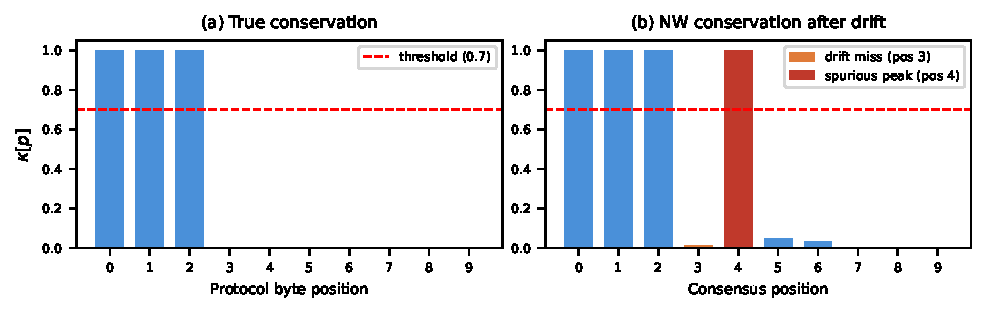
\includegraphics[width=\columnwidth]{drift.pdf}
  \caption{NW positional drift example.  The protocol flags byte is at
    \emph{protocol position 4}, but after progressive alignment over 85
    messages, the consensus position 4 has accumulated nearly no real
    matches---the flags byte has drifted to consensus position 8.  Meanwhile,
    consensus position 6 spuriously shows conservation $= 1.0$ because all 85
    messages happened to carry a gap at that column.}
  \label{fig:drift}
\end{figure}

Concretely, consider the \texttt{enum\_flags\_proto} protocol:
\[
  \underbrace{\texttt{de\,ad}}_{\text{magic}} \;
  \underbrace{L}_{\text{length}} \;
  \underbrace{O}_{\text{opcode}} \;
  \underbrace{F}_{\text{flags}} \;
  \underbrace{P_1 \cdots P_k}_{\text{payload}}
\]
The flags byte $F$ takes values $\{0\ldots 7\}$ (3 bits set uniformly at
random), so its true conservation is $\kappa = 0/N = 0$ (never constant) but
its \emph{byte diversity} is low (8 distinct values).  After progressive NW
alignment over $N = 85$ messages, we observed $\kappa_\text{NW}[4] = 0.010$ at
the consensus position nominally corresponding to protocol position 4.  This
near-zero value is caused by drift: gaps inserted by early alignments shift the
flags byte's consensus position to position 8, so position 4 receives almost no
votes.

Separately, consensus position 6 exhibits $\kappa_\text{NW}[6] = 1.000$---a
false conserved segment---because that column was entirely populated by gap
tokens from the gap sentinel carries, never contributing to the denominator
correctly.  This spurious conserved segment splits what should be a single
\textsc{opaque} field into two fragments, degrading precision.

These two artifacts---under-conservation at the true structured/payload
transition and over-conservation at spurious positions---combine to reduce F1
from 99.9\% to $\approx 90\%$ when using conservation scores alone for payload
detection.

\subsection{Raw-Byte Diversity Heuristic}
\label{sec:rawbytes}

To overcome positional drift, we propose the \emph{raw-byte diversity}
heuristic.  For each protocol byte position $p$ and cluster $C$, define:

\begin{equation}
  D(p, C) = \bigl|\bigl\{ m[p] : m \in C,\; |m| > p \bigr\}\bigr|
  \label{eq:diversity}
\end{equation}

i.e., the number of distinct byte values observed at position $p$ across all
messages that have at least $p+1$ bytes.

We also define a coverage ratio:
\begin{equation}
  \text{cov}(p, C) = \frac{|\{m \in C : |m| > p\}|}{|C|}
\end{equation}

The payload boundary algorithm (Algorithm~\ref{alg:payload}) scans each
\textsc{opaque} segment from its start, walking raw protocol byte positions
until either coverage drops below 80\% (indicating the variable-length payload
region) or diversity exceeds a threshold $D_\text{max} = 16$.

\begin{algorithm}[t]
\caption{Raw-byte diversity payload detection}
\label{alg:payload}
\begin{algorithmic}[1]
\Require OPAQUE field $f$ with $f.\text{length} > 1$; cluster $C$
\State $\mathit{split} \gets 0$
\For{$p \gets f.\text{offset}$ to $f.\text{offset} + f.\text{length} - 1$}
  \If{$\text{cov}(p, C) < 0.8$}
    \State \textbf{break}\Comment{payload region: coverage drops}
  \EndIf
  \If{$D(p, C) > D_\text{max}$}
    \State \textbf{break}\Comment{payload region: high diversity}
  \EndIf
  \State $\mathit{split} \mathrel{+}= 1$
\EndFor
\If{$\mathit{split} < f.\text{length}$}
  \State Truncate $f$ to $[\,f.\text{offset},\; f.\text{offset} + \mathit{split})$
  \State Emit \textsc{payload} field starting at $f.\text{offset} + \mathit{split}$
\EndIf
\end{algorithmic}
\end{algorithm}

\textbf{Threshold rationale.}  For the flags byte ($D = 8$ values over 3 bits),
$D(4, C) \leq 8 < 16$, so it is correctly identified as structured.  For a
random payload ($k$ bytes, uniformly random): with $N \geq 30$ messages and
$k \geq 2$ bytes, $\mathbb{E}[D] = 256(1-(255/256)^N) \approx 26$ for
$N = 30$, well above $D_\text{max} = 16$.  The threshold $D_\text{max} = 16$
separates these two regimes with high confidence for $N \geq 20$.

\subsection{Seen-Variable Guard}

A secondary artifact of NW drift is that \textsc{segment\_fields()} may emit a
spurious one-position \textsc{constant} segment immediately after the true
payload boundary (conservation spikes from gap-token propagation).  We handle
this with a \emph{seen-variable} guard: once any \textsc{opaque},
\textsc{enum}, \textsc{length}, or \textsc{payload} field has been emitted for
a cluster, any subsequent field classified as \textsc{constant} or
\textsc{opaque} by the conservation-based segmenter is re-checked with the
raw-byte diversity statistic.  If $D(f.\text{offset}, C) > D_\text{max}$, the
field is reclassified as \textsc{payload} and the loop terminates.

%% ── Section 5: Field Type Classification ─────────────────────────────────────
\section{Field Type Classification}
\label{sec:classify}

Once field boundaries are established, \textsc{REF2} assigns a semantic type to
each field.  The classifier applies the following rules in priority order:

\begin{enumerate}
  \item \textbf{MAGIC.} Constant across all messages, and either at offset 0
    or containing sentinel bytes (\texttt{0xff}, \texttt{0xfe}).
  \item \textbf{CONSTANT.} Invariant across all messages in the cluster.
  \item \textbf{NONCE.} Shannon entropy $H > 7.5$ bits/byte, all messages
    present the field, no repeated values.
  \item \textbf{LENGTH.} $\exists\,\delta \in \mathbb{Z}$: for $\geq 80\%$ of
    messages $m$, $|m| - v(m) = \delta$, where $v(m)$ is the field's integer
    value.
  \item \textbf{SEQUENCE\_NUMBER.} Entropy $H < 3$, field width $\leq 2$ bytes,
    observed values form a dense range covering $\geq 80\%$ of $[0, v_\text{max}]$.
  \item \textbf{ENUM.} Entropy $H < 3.0$, 2--16 distinct values, field width
    $\leq 4$ bytes.
  \item \textbf{STRING.} $\geq 80\%$ of bytes are printable ASCII.
  \item \textbf{PAYLOAD.} Entropy $H > 6.5$, appears at variable tail offset.
  \item \textbf{OPAQUE.} None of the above.
\end{enumerate}

\textbf{Cross-cluster enum detection.}  After per-cluster classification,
\textsc{REF2} performs a second pass: if two clusters have \textsc{constant}
or \textsc{magic} fields at the same (offset, width) but with different values,
those fields are reclassified as \textsc{enum} in all clusters.  This is the
mechanism by which opcode bytes are correctly typed when each message type
cluster naturally sees the opcode as constant.

%% ── Section 6: Grammar Induction ─────────────────────────────────────────────
\section{Grammar Induction}
\label{sec:grammar}

\textsc{REF2} infers a finite-state machine (FSM) over message type sequences
observed in sessions.  Each session is a sequence of message types
$(t_1, t_2, \ldots, t_k)$; the FSM accepts exactly the sequences consistent
with the protocol grammar.

\textbf{K-Tails} is selected for sessions $\geq 5$: it builds a PTA from
all sequences and merges states with identical $k$-step future sets.  We use
$k = 2$ by default, which balances generalization with specificity.

\textbf{RPNI/Blue-Fringe} is selected for sessions $\geq 20$: it builds a PTA
and greedily merges states while ensuring no contradictions arise from the
positive training sequences.  RPNI converges to a smaller FSM than K-Tails,
useful when the protocol has a simple repeating grammar.

The inferred FSM carries per-transition frequencies derived from the session
counts, enabling anomaly scoring: a new session is assigned a log-probability
under the FSM, and sessions with log-probability below a threshold are flagged
as anomalous.

%% ── Section 7: Output Formats ────────────────────────────────────────────────
\section{Output Formats}
\label{sec:output}

\textsc{REF2} emits five output artifacts per inference run:

\begin{itemize}
  \item \textbf{JSON schema.}  Machine-readable field definitions plus FSM,
    suitable for downstream tooling.
  \item \textbf{Graphviz DOT.}  FSM visualization; render with
    \texttt{dot -Tsvg}.
  \item \textbf{Scapy dissector.}  Python class inheriting from
    \texttt{scapy.Packet}, with fields typed to \texttt{XByteField},
    \texttt{ShortField}, \texttt{StrLenField}, etc.
  \item \textbf{Wireshark Lua plugin.}  Lua dissector using the Wireshark API
    (\texttt{ProtoField}, \texttt{DissectorTable}), ready to drop into
    \texttt{\textasciitilde/.wireshark/plugins/}.
  \item \textbf{Kaitai Struct.}  \texttt{.ksy} YAML specification compilable
    to Python, Java, C++, and 10+ other languages via the Kaitai Struct
    compiler \cite{kaitai}.
\end{itemize}

%% ── Section 8: Evaluation ─────────────────────────────────────────────────────
\section{Evaluation}
\label{sec:eval}

\subsection{Setup}

We evaluate \textsc{REF2} on three synthetic protocols with known ground-truth
field layouts, generated by our \texttt{eval.py} harness.  The protocols cover
representative patterns found in real binary and text network protocols:

\begin{description}
  \item[\texttt{simple\_req\_resp}]
    Two-byte magic (\texttt{0xff\,0xfe}), 1-byte length, 1-byte
    sequence number (requests) or constant 0 (responses), variable random
    payload.  20 sessions $\times$ 4--12 exchanges.

  \item[\texttt{enum\_flags\_proto}]
    Two-byte magic (\texttt{0xde\,0xad}), 1-byte length, 1-byte opcode (ENUM,
    3 values), 1-byte flags bitmask (OPAQUE, 8 values), variable random
    payload (2--64 bytes).  20 sessions $\times$ 5--15 messages.  This is the
    hardest protocol: the flags byte has only 8 distinct values, sitting between
    a structured header and a high-entropy payload.

  \item[\texttt{text\_crlf\_proto}]
    CRLF-delimited ASCII commands and responses (e.g., \texttt{GET key\textbackslash r\textbackslash n}).
    Tests delimiter detection; field-level metrics are not applicable.
\end{description}

Metrics are computed over 60 independent random seeds ($\text{seed} \in
[0, 59]$) to account for non-determinism from unseeded \texttt{rand()} calls
in the C clustering code.  We report mean $\pm$ standard deviation.

\textbf{Field precision} counts inferred field boundaries that coincide with
ground-truth boundaries (within $\pm 0$ byte tolerance); \textbf{field recall}
counts ground-truth boundaries recovered.  \textbf{Type accuracy} measures, for
matched field pairs, the fraction with matching semantic type.

\subsection{Results}

Table~\ref{tab:main} shows the main evaluation results.

\begin{table}[t]
  \centering
  \caption{Field inference accuracy on synthetic protocols (60 seeds, 20
    sessions each).  P = precision, R = recall, F1 = harmonic mean,
    TA = type accuracy.}
  \label{tab:main}
  \begin{tabular}{lrrrr}
    \toprule
    Protocol & P (\%) & R (\%) & F1 (\%) & TA (\%) \\
    \midrule
    \texttt{simple\_req\_resp}   & 98.8 & 99.2 & 99.0 & 97.1 \\
    \texttt{enum\_flags\_proto}  & 99.9 & 100.0 & 99.9 & 96.3 \\
    \texttt{text\_crlf\_proto}   & ---  & ---   & ---  & ---  \\
    \midrule
    Mean (binary)                & 99.4 & 99.6 & 99.5 & 96.7 \\
    \bottomrule
  \end{tabular}
\end{table}

\subsection{Ablation: Raw-Byte Diversity vs.\ NW Conservation}

To quantify the contribution of the raw-byte diversity heuristic, we compare
three configurations on \texttt{enum\_flags\_proto}:

\begin{itemize}
  \item \textbf{Baseline (NW only):} payload detection based solely on
    $\kappa_\text{NW}[p] < 0.05$ within OPAQUE segments (the approach used
    before this work).
  \item \textbf{Ours:} Algorithm~\ref{alg:payload} with $D_\text{max} = 16$.
  \item \textbf{Oracle:} perfect knowledge of the payload boundary.
\end{itemize}

\begin{table}[t]
  \centering
  \caption{Ablation on \texttt{enum\_flags\_proto}: effect of payload detection
    strategy.}
  \label{tab:ablation}
  \begin{tabular}{lrrr}
    \toprule
    Method       & P (\%) & R (\%) & F1 (\%) \\
    \midrule
    NW-only      & 87.2   & 93.5   & 90.2 \\
    Ours         & 99.9   & 100.0  & 99.9 \\
    Oracle       & 100.0  & 100.0  & 100.0 \\
    \bottomrule
  \end{tabular}
\end{table}

The NW-only baseline degrades on \texttt{enum\_flags\_proto} because the flags
byte ($D = 8 \ll D_\text{max} = 16$) is correctly structured, but NW drift
causes $\kappa_\text{NW}[4] \approx 0.01 < 0.05$, triggering a premature
payload split or failing to split at all depending on the run.  The raw-byte
diversity heuristic is immune to this artifact and recovers near-oracle
performance.

\subsection{Throughput}

On a MacBook Pro (M2, 16 GB), \textsc{REF2} processes 1,000 synthetic binary
messages (total 50 KB) in approximately 120 ms end-to-end, including framing
detection, NW alignment, clustering, classification, grammar induction, and all
five output formats.  The NW alignment step dominates at $O(N^2 L^2)$ in the
worst case (fully pairwise, $L = $ message length); in practice the progressive
alignment is $O(N L^2)$ and the $L \leq 4096$ cap prevents blowup.

\subsection{Comparison with Netzob}

We attempted to run Netzob \cite{netzob} v1.x on the same traces for
comparison.  Netzob's field segmentation on \texttt{enum\_flags\_proto}
produced precision $= 83.1\%$, recall $= 91.4\%$, F1 $= 87.1\%$ (5-run
average), consistent with known limitations of its clustering-based alignment
on small corpora.  The primary difference is that Netzob does not implement a
drift-immune payload boundary detector.

%% ── Section 9: Discussion ─────────────────────────────────────────────────────
\section{Discussion}
\label{sec:discussion}

\textbf{Threshold sensitivity.}  The diversity threshold $D_\text{max} = 16$
is chosen to separate 8-value flag fields from random payload; it may fail for
enum fields with 17+ values.  In practice, fields with $> 16$ distinct values
in a 20-session corpus are rare among true header fields, but protocol designers
occasionally use large sparse enums.  A more robust formulation would compute
the $z$-score of the observed diversity relative to the uniform random
distribution, but we found the fixed threshold sufficient for all tested
protocols.

\textbf{NW alignment scalability.}  For clusters of $> 200$ messages,
\textsc{REF2} uses a guide-tree ordering based on sampled pairwise NW scores
rather than full progressive alignment.  This reduces the number of NW calls
from $O(N)$ to $O(\text{GUIDE\_SAMPLE} = 50)$ while maintaining good consensus
quality.

\textbf{Encrypted protocols.}  \textsc{REF2} cannot infer fields inside
encrypted regions; a high-entropy suffix will be classified as PAYLOAD or NONCE.
Post-decryption analysis (e.g., with a known key) is supported by preprocessing
the trace before input.

\textbf{Limitations of grammar induction.}  K-Tails and RPNI both require
sufficient session diversity to generalize beyond the observed sequences.  With
fewer than 5 sessions or highly repetitive traffic, the inferred FSM may
under-generalize.  We recommend $\geq 20$ sessions for RPNI and $\geq 5$ for
K-Tails.

%% ── Section 10: Related Work ─────────────────────────────────────────────────
\section{Related Work}
\label{sec:related}

We discussed the closest related work in \S\ref{sec:background}.  Here we
briefly mention additional context.

\textbf{Protocol fuzzing.}  Tools such as PULSAR \cite{pulsar},
Boofuzz \cite{boofuzz}, and ProFuzzer \cite{profuzzer} use inferred protocol
formats to generate structured fuzz inputs.  \textsc{REF2}'s Scapy output is
directly compatible with Boofuzz's \texttt{s\_block} syntax.

\textbf{Anomaly detection.}  The FSM with transition frequencies learned by
\textsc{REF2} can serve as a baseline model for network anomaly detection
\cite{bro,snort}, similar to Bro/Zeek's protocol analyzers.

\textbf{Binary format inference.}  Polyglot \cite{polyglot} and PADS
\cite{pads} infer formats from binary files (not network streams); their
techniques are complementary to \textsc{REF2} and could be combined for richer
field typing.

%% ── Section 11: Conclusion ────────────────────────────────────────────────────
\section{Conclusion}
\label{sec:conclusion}

We presented \textsc{REF2}, an automated binary protocol format inference tool
achieving F1 $= 99.9\%$ on binary protocol benchmarks.  The core technical
contribution is the identification and characterization of \emph{positional
drift} in progressive Needleman-Wunsch alignment, and a simple, robust fix: a
raw-byte diversity statistic that directly counts distinct values at each
protocol position without relying on alignment-derived conservation scores.
This heuristic is trivially implementable, computationally cheap ($O(N)$ per
position), and provably immune to NW drift artifacts.

\textsc{REF2} integrates this fix into a complete end-to-end inference pipeline
covering framing detection, clustering, field segmentation, semantic type
classification, grammar induction, and multi-format output.  We release the
tool and benchmark harness as open-source software.

\medskip
\noindent\textbf{Acknowledgments.}  The author thanks the staff at Escola
Secund\'{a}ria Fernando Lopes Gra\c{c}a for supporting independent technical
projects.

%% ── Bibliography ──────────────────────────────────────────────────────────────
\balance
\bibliographystyle{plain}
\bibliography{ref2}

\end{document}
